\chapter{Experimental System and Setup}
Because of the issues with stimuli generation the experiment setup has not been
employed on live neural tissue.
As a consequence, the current experimental setup is designed to be easy to
modify whenever testing becomes possible and to verify functionality of the rest
of the system.
Consequentially, the focus on this section is the experimental capabilities
provided by the system and the parameter space that can be explored.
When leaving out all implementation details the experimental setup provided by
SHODAN and MEAME becomes much simpler, as shown in \ref{figExperimentLoop}.
The figure highlights a point mentioned in the previos section, namely that the
closed loop system actually consists of two data-loops running in parallel.
This is a departure from the classical reservoir computer model where
modifications are made between runs.
In the classic model experiments are run, performance is evaluated and the
readout layer is altered in some way.
This mode of operation makes sense when the reservoir can be reset to an initial
state, but as discussed this is not possible when dealing with neural tissue
which evolve both short term and long term.
The experiment setup from \ref{figExperimentLoop} can be broken up into three
parts: The data loop, the core reservoir computer and the reconfiguration loop.
The three following section gives a brief description of purpose and which
parameters can be altered.
To give a better overview these parameters are then summarized in the subsequent
section.
\begin{figure}[h!]
  \centering
  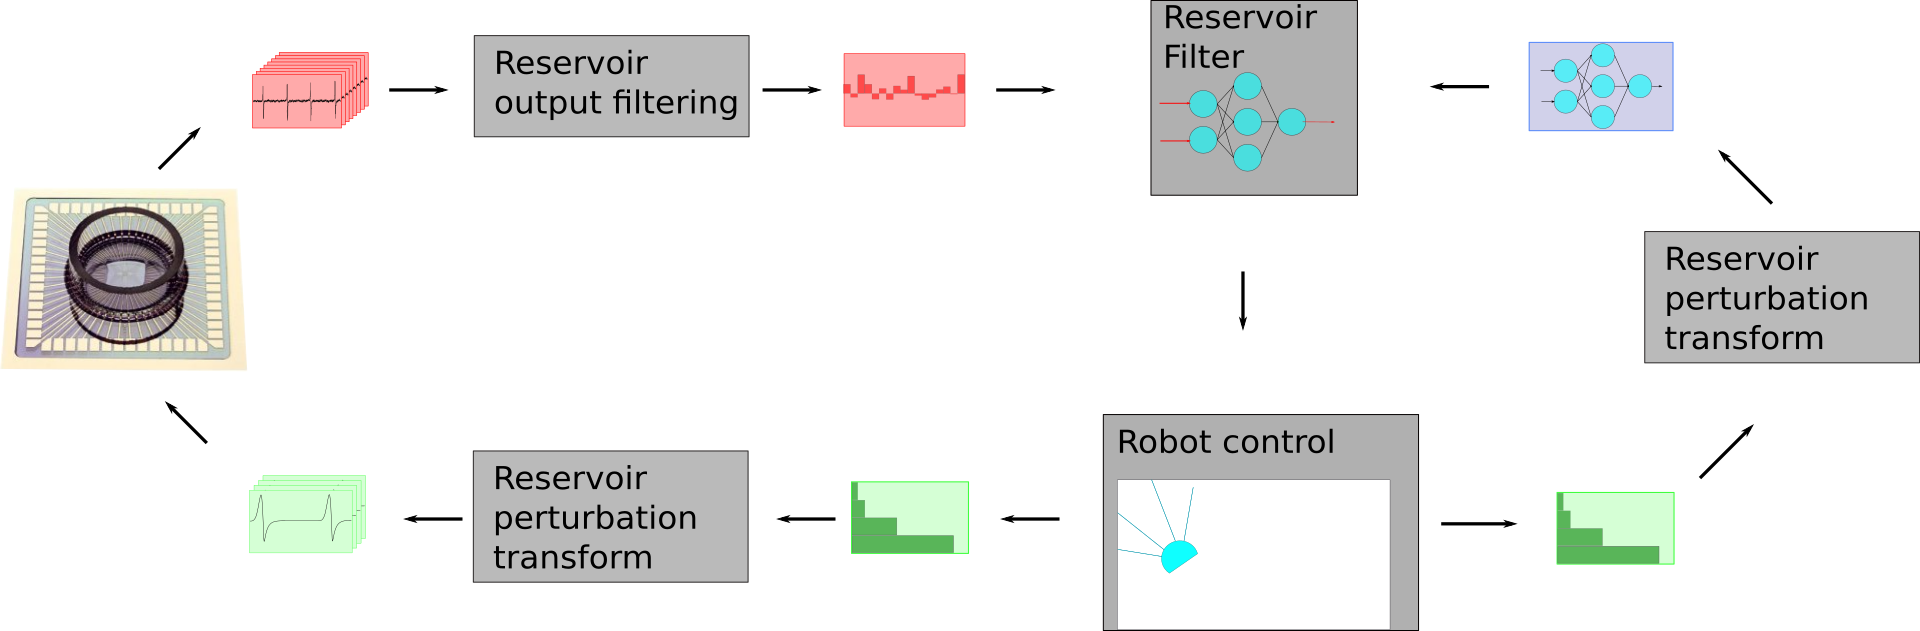
\includegraphics[width=0.5\textwidth]{fig/experimentLoop.png}
  \caption{Rough sketch.
    Some wavez
  }
  \label{figExperimentLoop}
\end{figure}
%
\section{Data Loop}
A closer look at the data loop is shown in figure \ref{figDataLoop}.
The two ``knobs'' that can be turned in this part of the system is the reservoir
input filter and the perturbation transform.
The reservoir output filtering module, as discussed in the previous chapter,
perform a spike detection which is then used as input to an averaging filter.
While the spike detection is considered to be fixed, the averaging filter is
not.
In the current implementation it is a simple averaging filter, but it can easily
be changed to use a different model, such as linear of exponential decay if the
averaging filter is deemed insufficient.
The second module is the reservouir perturbation transform which transforms a
set of distances perceived by the robot into stimulus frequencies.
The perturbation model has three parameters: A list of electrodes to receive the
stimulus signal, the period between applying stimuli, and the stimuli signal
itself.
Much like the choice of using a simple averaging filter, the default settings
for the perturbation transform favors simplicity.
For each sensor on the robot a single electrode is chosen and is generally
considered outside the interesting parameter space.
Similarily a simple waveform is chosen, either a sine wave or a square wave.
These samples are fixed, increasing the period means there will be a longer
period between each sample, but the samples themseleves remain fixed.
Again, for simplicity, a simple square wave is the default choice, thus the only
parameter that is not considered fixed is the transform between distance and
period.
The chosen default for this transform is an exponential decay, when the sensor
is facing a wall directly the square stimuli frequency is set to $30hz$ with an
exponential dropoff to $1/3hz$ when the sensor perceives a wall at the maximum
distance.
\begin{figure}[h!]
  \centering
  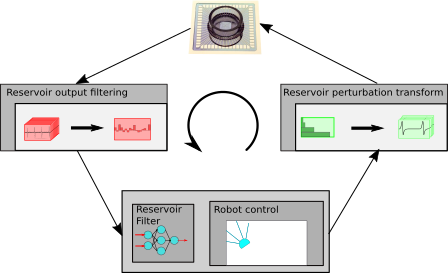
\includegraphics[width=0.5\textwidth]{fig/RCloop.png}
  \caption{Rough sketch.
    Some wavez
  }
  \label{figDataLoop}
\end{figure}
%
\section{Core Reservoir Computer}
As discussed in the previous chapter, the core reservoir computer is the
ideal reservoir readout layer and the perturbation generator while the remaining
functionality is abstracted away in the interface and feedback processor box.
The core reservoir computer consists of two parts, the robot control and the
reservoir readout layer.
\subsubsection{Readout Layer}
The chosen readout layer is a simple feed forward neural network.
As mentioned in the background, the choice of using a network with multiple
layers as indicated in the figure means that a non-linear problem may be solved
entirely by the readout layer.
For the proof of concept the topology of the network is not fixed to a topology,
thus it is up to the experimenter whether a network with a single layer or one
with multiple layers should be used.
In fact, there is no strict requirement that the readout layer must be an
artificial neural network at all.
While it might seem a wise choice to use a readout layer that has similarities
with the reservoir itself, this line of thinking ignores the ``anonymization''
that happens between reservoir and reservoir computer, as shown in the fig
\ref{figGenericSpecific} in the previous chapter.
The final word on the choice of readout layer is that the artificial neural
network approach has the following benefits:
It can easily be extended from a linear to nonlinear classifier, and it is easy
to modify during an experiment.
\subsubsection{Robot Control}
The robot control is a simulator that controls an agent with 4 ``eyes'' in a box
world as shown in \ref{figGame}.
As with all other parts of the system variables such as the amount of eyes, sight
range, the function between the output of the reservoir filter and robot
movement, max turn rate and max speed can be changed on a per-experiment basis.
The goal of the ``game'' is for the robot to not collide with walls.
Since the best way to avoid this is to simply run in circles, the performance is
evaluated by how close the agent came to crashing in a series of trials where
the agent is faced towards the wall at different angles as shown in fig [TODO].
Since the actions of the robot are decided by the output of the readout layer it
the action of the agent indirectly depends on the evaluation function since it
is this evaluation that shapes the next readout layer.
\begin{figure}[h!]
  \centering
  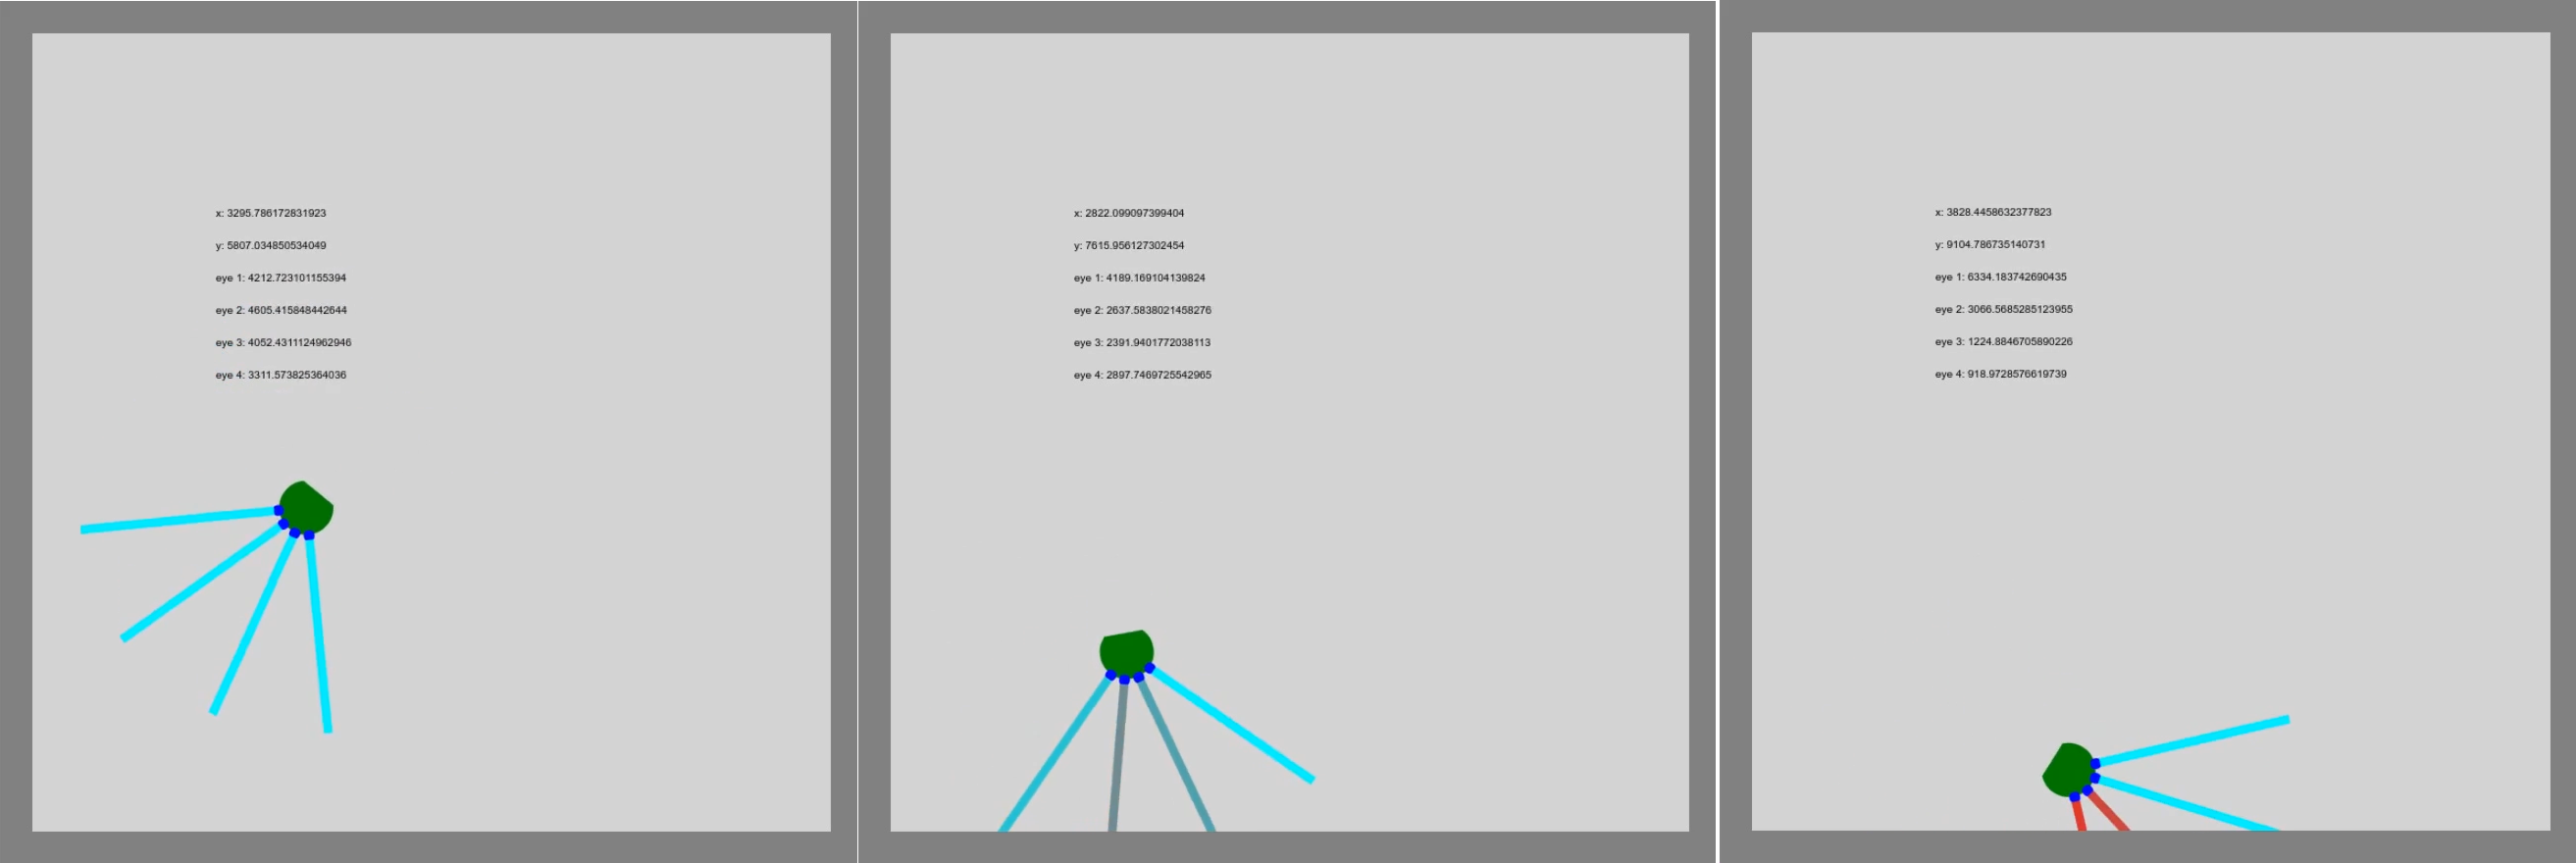
\includegraphics[width=1\textwidth]{fig/TAC/game2.png}
  \caption{The cyborg doing its thing}
  \label{figGame}
\end{figure}
\begin{figure}[h!]
  \centering
  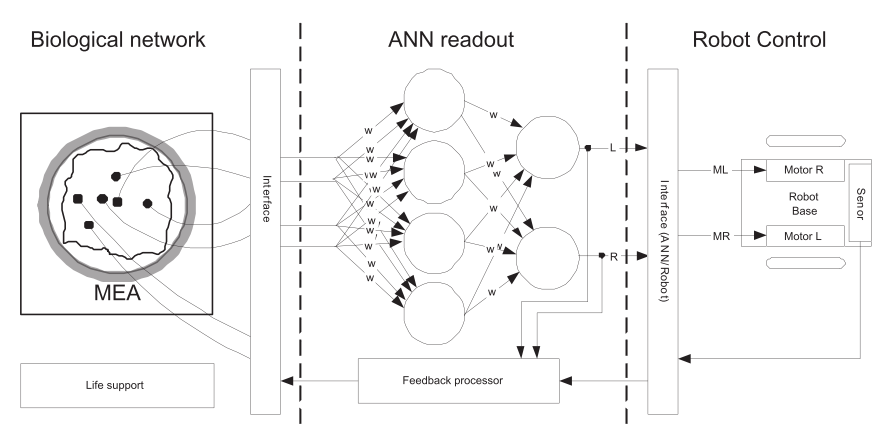
\includegraphics[width=1\textwidth]{fig/cyborg_overview.png}
  \caption{A simple conceptual cyborg.}
  \label{cyborgOverviewSimple}
\end{figure}
\section{Reconfiguration Loop}
The reconfiguration loop, shown in \ref{figReconfLoop} is the dataflow
responsible for the on-line reconfiguration of the reservoir readout layer.
On experiment start the reservoir filter reconfigurator supplies the readout
layer module with a set of weights for the artificial neural network and records
the resulting behavior.
Each attempt is scored according to a scoring function as described in the
previous section, and from this the reservoir filter reconfigurator generates
new readout layers.
The chosen method of readout layer generation is a \emph{genetic algorith}
because of its ease of implementation and relative lack of bias.
\begin{figure}[h!]
  \centering
  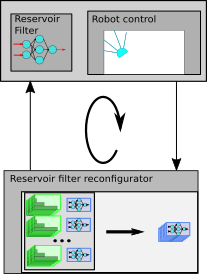
\includegraphics[width=0.5\textwidth]{fig/reconfigLoop.png}
  \caption{Rough sketch.
    Some wavez
  }
  \label{figReconfLoop}
\end{figure}
\section{Parameter Space}
The first distinction in the parameter space is 


\cleardoublepage

%%% Local Variables:
%%% mode: latex
%%% TeX-master: "../main"
%%% End:
